\chapter{Aufgabe 3}

\section{Teil 1}

\textit{Erstellen Sie eine Wahrheitstabelle für eine Digitalschaltung, die das Paritätsbit (bei gerader Parität) berechnet.
Wir gehen im Folgenden davon aus, dass vier Bits übertragen werden sollen,  die durch eine Digitalschaltung mit einem Paritätsbit ergänzt werden sollen.} \\

\noindent
Beispiel für ein Wort (4 Bit, + 1 Paritätsbit), das, unter Angabe gerader Parität, als korrekt übertragen gilt:

\begin{equation}\notag
    \texttt{0 0 0 0 | 0}
\end{equation}

\noindent
Das zu übertragende Wort besteht aus $4$ Bit, die allesamt auf $0$ gesetzt sind.\\
Die Anzahl der $1$en in dem Wort ist \textit{gerade} (da $2|0$).\\
In dem Fall muss das Paritätsbit (bei \textit{gerader} Parität) ebenfalls auf $0$ gesetzt werden, denn

\begin{itemize}
    \itemsep0.5em
    \item wird statt der \texttt{0 0 0 0} bspw. \texttt{0 1 0 0} übertragen (Informationswort \texttt{0 1 0 0 | 0}), ist die Anzahl der übertragenen $1$en in dem Wort \textit{ungerade}, das Paritätsbit müsste demnach auf $1$ gesetzt sein, ist aber auf $0$ gesetzt
    \item ist das Wort \texttt{0 0 0 0} und das Paritätsbit $1$ (das Informationswort also \texttt{0 0 0 0 | 1}), gilt das Signal ebenfalls als fehlerhaft, da nun wieder eine ungerade Anzahl von $1$en übertragen wurde, das Paritätsbit aber eine gerade Anzahl an $1$en erwartet.
\end{itemize}

\noindent
Beispiel für ein Wort ($4$ Bit) mit ungerader Anzahl von $1$en, + Paritätsbit:

\begin{itemize}
    \itemsep0.5em
    \item \texttt{0 1 0 0 | 1}: korrekt, da insgesamt $2$ Bit auf $1$ gesetzt sind - inkl. Paritätsbit
    \item \texttt{0 1 0 1 | 1}: fehlerhaft, Paritätsbit gibt an, dass gerade Anzahl an $1$en erwartet wurde, es finden sich aber $3$ Bit in dem Informationswort, die jeweils auf $1$ gesetzt sind.
\end{itemize}

\noindent
Insgesamt ergibt sich damit Kombination der Eingangssignale mit dem jeweils berechneten Paritätsbit wie in Tabelle~\ref{tab:paritätsbit} angegeben.


\begin{table}[ht]
    \setlength{\tabcolsep}{0.5em}
    \def\arraystretch{1.5}
    \centering
   \begin{tabular}{|c|c|c|c|c||c|}
        \hline
        \textbf{Zeile} & $A_3$ & $A_2$ & $A_1$ & $A_0$ & $y$ \\
        \hline \hline
        0  & 0 & 0 & 0 & 0 & 0 \\ \hline
        1  & 0 & 0 & 0 & 1 & 1 \\ \hline
        2  & 0 & 0 & 1 & 0 & 1 \\ \hline
        3  & 0 & 0 & 1 & 1 & 0 \\ \hline
        4  & 0 & 1 & 0 & 0 & 1 \\ \hline
        5  & 0 & 1 & 0 & 1 & 0 \\ \hline
        6  & 0 & 1 & 1 & 0 & 0 \\ \hline
        7  & 0 & 1 & 1 & 1 & 1 \\ \hline
        8  & 1 & 0 & 0 & 0 & 1 \\ \hline
        9  & 1 & 0 & 0 & 1 & 0 \\ \hline
        10 & 1 & 0 & 1 & 0 & 0 \\ \hline
        11 & 1 & 0 & 1 & 1 & 1 \\ \hline
        12 & 1 & 1 & 0 & 0 & 0 \\ \hline
        13 & 1 & 1 & 0 & 1 & 1 \\ \hline
        14 & 1 & 1 & 1 & 0 & 1 \\ \hline
        15 & 1 & 1 & 1 & 1 & 0 \\
        \hline
    \end{tabular}
    \caption{Lösungsvorschlag für Aufgabe 3.1}
    \label{tab:paritätsbit}
\end{table}

\section{Teil 2}

\textit{Erstellen Sie das zugehörige KV-Diagramm.
Versuchen Sie, die Schaltfunktionen zu vereinfachen, indem Sie benachbarte Eins-Felder zu Blöcken zusammenzufassen. Markieren Sie diese Blöcke im KV-Diagramm.}\\

\noindent
Das KV-Diagramm ist in Abbildung~\ref{fig:kv_parität} angegeben.\\
Es zeigt sich, dass keine Blöcke zusammengefasst werden können.


\begin{figure}
    \centering
    \includegraphics[scale=0.5]{aufgabe 3/img/kv_parität.svg}
    \caption{KV-Diagramm für Aufgabe 3.2. Tiefgestellte Ziffern beziehen sich auf die zugehörigen Zeilen in Tabelle~\ref{tab:paritätsbit}.  (Quelle: eigene)}
    \label{fig:kv_parität}
\end{figure}

\section{Teil 3}

\textit{Geben Sie eine Schaltung an, die die (gerade) Parität für das Datenwort  0001 generiert.}\\

\noindent
Die Schaltung für die Funktion $\neg A_3 \land \neg A_2 \land \neg A_1 \land A_0$ ist in Abbildung~\ref{fig:schaltplan_parität} angegeben.

\begin{figure}
    \centering
    \includegraphics[scale=0.6]{aufgabe 3/img/schaltplan_parität.svg}
    \caption{Schaltung für die Funktion $\neg A_3 \land \neg A_2 \land \neg A_1 \land A_0$ aus Aufgabe 3.3. Der Übersicht halber sind wieder mehrere Gatter zusammengefasst, wo angebracht. (Quelle: eigene)}
    \label{fig:schaltplan_parität}
\end{figure}

\section{Teil 4}

\textit{Suchen Sie im Internet nach einem Datenblatt des SN74150 und stellen
Sie fest,\\
    (1) wie viele Eingänge der SN74150 besitzt,\\
    (2) wie die Eingangspegel auf den Ausgang W übertragen werden und\\
    (3) welche Bedeutung der Pin 9 (strobe) besitzt.
}\\

\noindent
Laut dem Datenblatt des SN74150\footnote{
Quelle: \url{https://www.alldatasheetde.com/datasheet-pdf/download/204647/TI/SN74150.html}, abgerufen 24.03.2025
}

\begin{enumerate}
    \itemsep0.5em
    \item hat der Multiplexer 16 Eingänge (E0 - E15)
    \item werden die Eingangspegel $D, C, B, A$ auf den Ausgang $W$ übertragen, und der Wert entspricht dem Komplement des Signals, das an EN (N = $[0..15]$) anliegt. \\
    Bspw. ist (informell) $(D = L) \land  (C = L) \land (B = L) \land (A = L) \implies \neg E0$, wobei $L$ für \textit{low level} steht.
    Berücksichtigt wird hierbei noch der Pin 9, der für \ldots
    \item \ldots \texttt{strobe} steht: ``[\ldots] a strobe input which must be at a low logic level to enable these devices``\footnote{
    Zitat aus dem ang. Dokument
    }.
    Daraus lässt sich ableiten, das an dem Ping keine Spannung anliegen darf, damit die Adresseingänge $D, C, B, A$ die entsprechenden Inputs $E0..E15$ durchschalten können.
\end{enumerate}

\section{Teil 5}

\textit{Wenn Sie den Multiplexer SN74150 zur Generierung eines (geraden)
Paritätsbits einsetzen, tragen Sie bitte in die Abbildung ein, wie Sie\\
(1) die Eingänge (Data Inputs),\\
(2) die Adresseingänge (DCBA)\\
(3) und den Strobe-Eingang beschalten würden.}\\

\noindent
Die Abbildung mit der vorgeschlagenen Beschaltung ist in Abbildung~\ref{fig:multiplexer} dargestellt.

\begin{enumerate}
    \itemsep0.5em
    \item Die Eingänge $In_0, In_1, \ldots In_{15}$ ``entsprechen`` zeilenweise dem jeweiligen $y$ aus Tabelle~\ref{tab:paritätsbit} -
    da die Eingänge allerdings negiert an $W$ ausgegeben werden, müssen diese \textit{negiert} als Eingaben angelegt werden, also
     $In_i = \neg y_i$, mit $i \in [0..15]$ ($i$ ist Zeilenindex, also $i = (A_3 A_2 A_1 A_0)_2$).
    \item An den Data Inputs $D, C, B, A$  liegen entsprechend die Werte für $A_3, A_2, A_1, A_0$ an (s. Tabelle~\ref{tab:paritätsbit}), also $2^4$ Kombinationen von \textit{low level input} (= 0) und \textit{high level input} (= 1).
    \item An dem \texttt{strobe} Eingang muss \textit{low level input} anliegen
\end{enumerate}

\begin{figure}
    \centering
    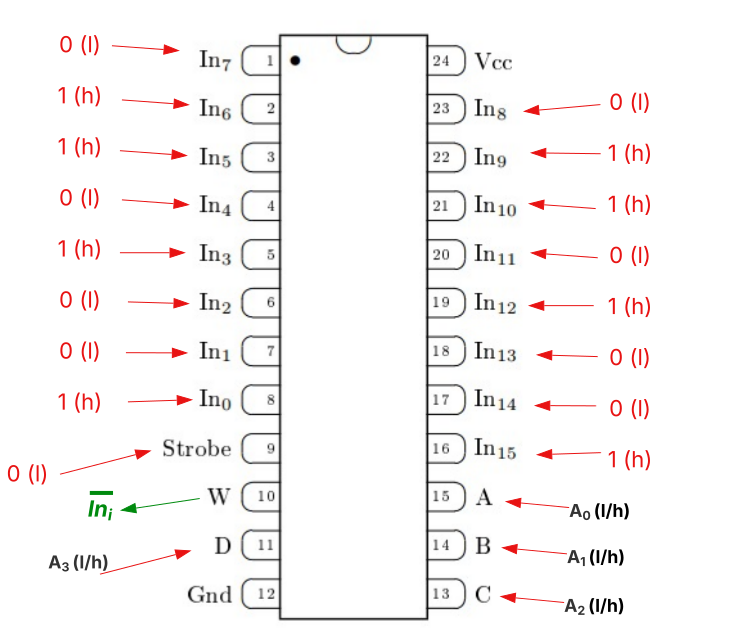
\includegraphics[scale=0.5]{aufgabe 3/img/multiplexer.svg}
    \caption{Schematische Darstellung der Beschaltung eines SN74150 Multiplexers zur Ausgabe eines Paritätsbits basierend auf Tabelle~\ref{tab:paritätsbit}. (Quelle: eigene, Pinbelegung aus Einsendeaufgaben 1, Abbildung 14)}
    \label{fig:multiplexer}
\end{figure}